%!TEX TS-program = pdflatex
%!TEX root = progetto_finale.tex
%!TEX encoding = UTF-8 Unicode

\chapter{Progetto} \label{progetto}

In questo capitolo vengono descritte l'architettura del software, i protocolli e gli algoritmi utilizzati, l'architettura fisica e il piano di sviluppo.

This chapter is devoted to the description of the general architectures, and specific algorithms.

\section{Architettura Logica}
Describe the components of your systems: modules/objects/components/services. For each component, describe the functionalities it implements, and by who is used.

\begin{itemize}
	\item Modulo algoritmi grafi: fornisce gli algoritmi che è possibile utilizzare sui grafi. Per esempio include Dijkstra, BFS, DFS, aggiungi nodo, aggiungi arco, ... 
	
	\item Modulo per l'algoritmo di elezione del leader: implementa la funzionalità della scelta della macchina da assegnare all'utente.
	
	\item Modulo per l'invio di messaggi: controlla che il messaggio sia ben formato.
	
	\item Modulo interfaccia cliente-servizio: fornisce le possibili operazioni che un cliente può richiedere al sistema.
	
	\item Modulo scheda wireless: simula la scheda di rete che fornisce i vicini dell'entità che ne invoca i metodi.
	
	\item Modulo mappa città: fornisce i metodi di lettura e modifica della mappa della città.
	
	\item Modulo gestione macchine: fornisce i metodi per ricaricare le batterie delle macchine, ne gestiscono gli incidenti e le riparazioni.
	
	\item Modulo creazione entità: fornisce le primitive per creare nuove macchine e nuovi utenti.
	
	\item Modulo comunicazione Ambiente-Entità: il processo Ambiente può utilizzare i metodi in questo modulo per simulare il mondo reale.
	
	\item Modulo Entità Macchina: rappresenta l'astrazione dell'entità veicolo.
	
	\item Modulo Entità Utente: rappresenta l'astrazione dell'entità utente.

\end{itemize}

Per rappresentare il comportamento delle entità coinvolte in base ai possibili eventi, sono stati creati due automi che rappresentano i possibili stati delle macchine e degli utenti. In essi, gli stati sono rappresentati da degli ovali, mentre gli eventi da dei riquadri di colore blu o rosso. Queste tonalità esprimono il tipo di messaggio: ricezione ed invio.

L'immagine \ref{fig:automa_utente} rappresenta l'automa degli stati dell'entità utente e come esso cambia il proprio stato in base agli eventi e messaggi.


\begin{figure}[htbp]
	\centering
	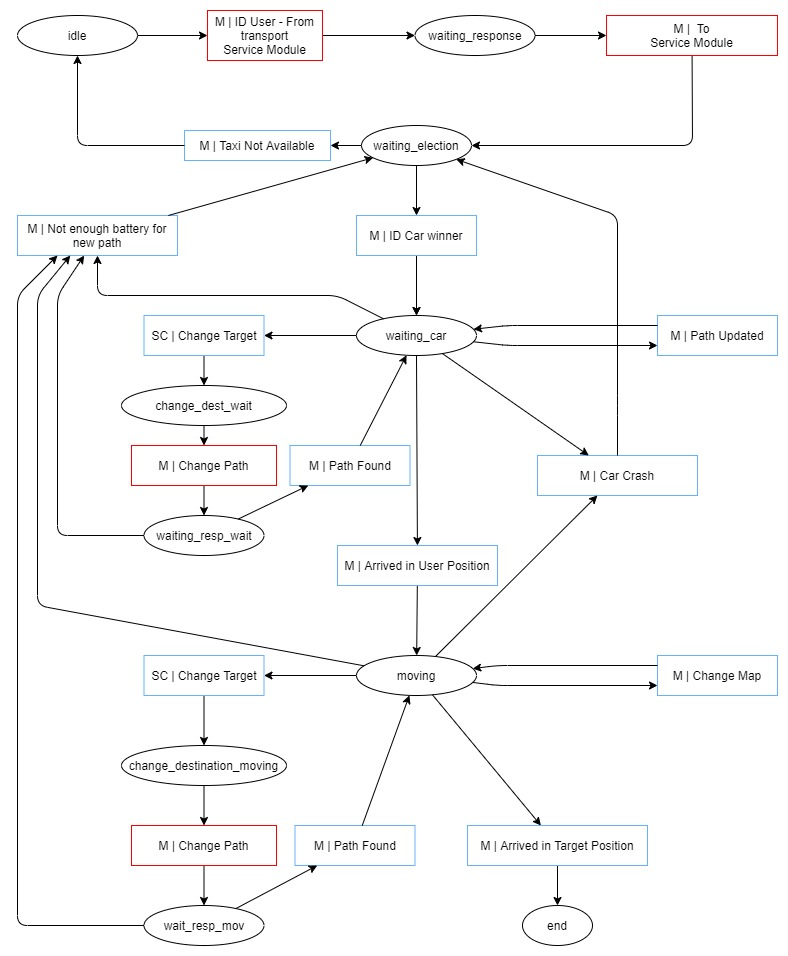
\includegraphics[width=15cm]{automa_utente.jpg}
	\caption{Rappresentazione degli stati possibili dell'entità utente.}
	\label{fig:automa_utente}
\end{figure}

L'immagine \ref{fig:automa_macchina} rappresenta l'automa degli stati dell'entità macchina e come esso cambia il proprio stato in base agli eventi e messaggi.


\begin{figure}[htbp]
	\centering
	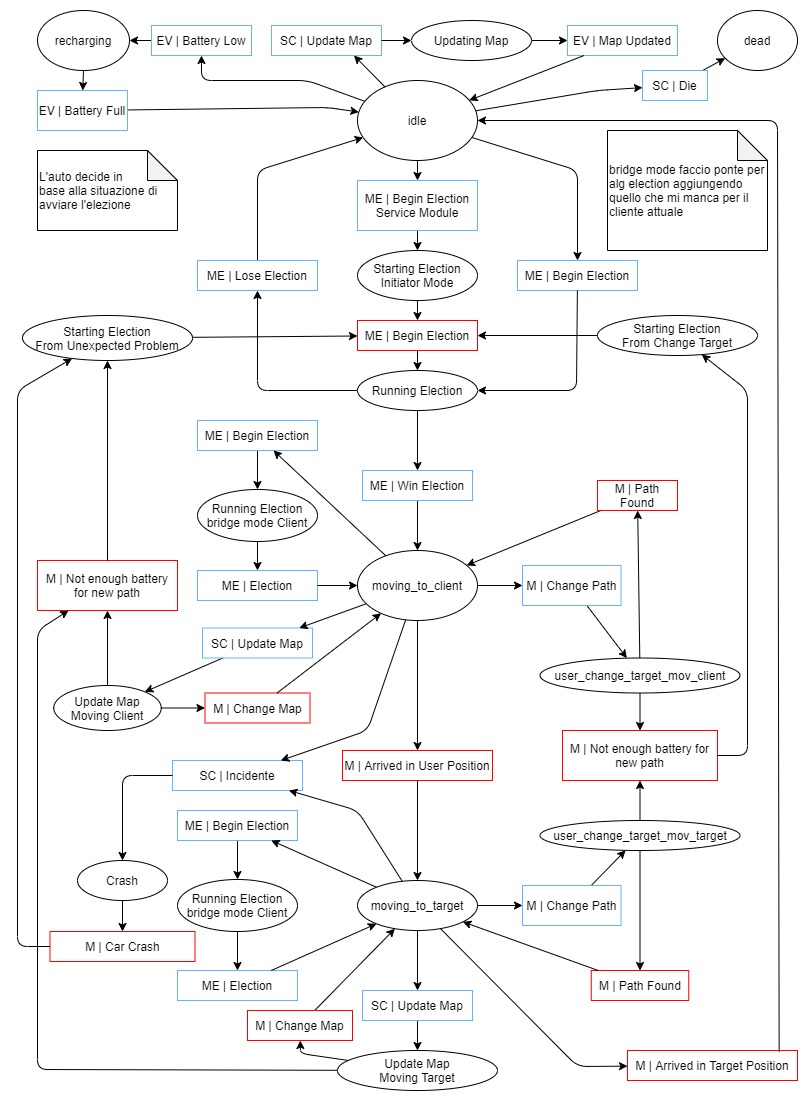
\includegraphics[width=15cm]{automa_macchina.jpg}
	\caption{Rappresentazione degli stati possibili dell'entità macchina.}
	\label{fig:automa_macchina}
\end{figure}

\newpage

\section{Protocolli e algoritmi}
Communication between components. UML sequence diagrams go here. Also, put here a detailed description of distributed algorithms used to solve specific problems of the project.

\subsection{Algoritmo di Elezione}
per l'elezione

\subsection{Diagrammi di sequenza dei messaggi}
All'appendice \ref{messaggi_scambiati_appendix}, sono presenti i diagrammi di sequenza dei messaggi che vengono scambiati tra i diversi moduli per permettere le funzionalità del sistema.

\begin{itemize}
	\item Movimento del taxi alla posizione dell'utente e successivo trasporto \ref{fig:messaggi_utente_trasporto}.
	\item Richiesta da parte dell'utente del servizio di trasporto \ref{fig:messaggi_utente_chiede_macchina}.
	\item Richiesta di cambiamento di destinazione da parte dell'utente mentre il taxi è in viaggio verso l'utente \ref{fig:messaggi_utente_cambio_direzione_waiting}.
	\item Richiesta di cambiamento di destinazione da parte dell'utente mentre il taxi lo sta trasportando \ref{fig:messaggi_utente_cambio_direzione_moving}.
	\item Partecipazione all'elezione di una macchina non iniziatrice \ref{fig:messaggi_macchina_partecipazione_elezione}. Poiché è possibile che la macchina si trovi in diversi stati mentre viene avviato l'algoritmo di elezione, sono stati rappresentati tre possibili scenari.
	\item Incidente di una macchina con conseguente notifica all'utente e ricerca di un taxi alternativo \ref{fig:messaggi_macchina_crash}.
	\item Ricarica della macchina, rimozione della macchina dal sistema e aggiornamento della mappa  \ref{fig:messaggi_macchina_batteria_morte_mappaIdle}. In queste operazioni si considera che la macchina sia nello stato 'idle'.
	\item Aggiornamento della mappa della città mentre il taxi si sta muovendo verso il cliente \ref{fig:messaggi_macchina_aggiornamento_mappa_to_client}.
	\item Aggiornamento della mappa della città mentre il taxi sta trasportando il cliente a destinazione \ref{fig:messaggi_macchina_aggiornamento_mappa_to_target}.
\end{itemize}


\section{Architettura fisica e Distribuzione}
Per l'implementazione fisica del progetto, è necessario che ogni automobile elettrica sia dotata di una scheda Wi-Fi per la comunicazione con i veicoli vicini. Il cliente per poter comunicare con il sistema necessita di utilizzare un'applicazione dedicata per le prenotazioni. Si suppone esista già la mappa della città nel formato adatto, ogni automobile deve possederne una copia nel disco locale. Un altro requisito hardware è che le macchine dispongano di sufficiente potenza di calcolo per effettuare velocemente il calcolo dei percorsi.

% Which nodes and platforms involved, and where each component is deployed.

\section{Piano di Sviluppo}
% Since it is diffcult to predict just how hard implementing a new system will be, you should formulate as a set of "tiers", where the basic tier is something youre sure you can complete, and the additional tiers add more features, at both the application and the system level.

Sono stati individuati due insiemi di funzionalità che è necessario supportare.
\subsection{Funzionalità Base}

\begin{enumerate}
%	\item Panino alla guida
	\item Comunicazione peer to peer per la leader election.
	\item Richiesta dell'utente di trasporto.
	\item Gestione della ricarica delle macchine.
	\item Cambio di direzione.
	\item Gestione degli incidenti sia delle macchine che delle strade rotte.
\end{enumerate}

\subsection{Funzionalità Aggiuntive}

\begin{itemize}
	\item Lista di possibili taxi in caso di pareggio tra i candidati.
	\item Perdita delle connessioni mentre si elegge il leader.
	\item Partecipazione della macchina già impegnata alla leader election.
	\item Car sharing fino a tre persone.
\end{itemize}

\subsection{Ordine di sviluppo}
Lo sviluppo dell'applicazione verrà suddiviso in diverse versioni via via estese con le nuove funzionalità. In particolare si seguirà questo ordine:

\begin{enumerate}
	\item Ogni macchina potrà parlare con tutte le altre macchine; l'utente invia la richiesta di trasporto alla macchina più vicina a lui; se un veicolo è impegnato con un cliente non partecipa alla selezione del leader per il trasporto; la comunicazione tra i veicoli è diretta, quindi ogni taxi può parlare con chiunque.
	\item Vengono aggiunte le colonnine di ricarica, alle quali le macchine devono far rifornimento se hanno esaurito le batterie; le macchine possono guastarsi; l'utente può decidere di cambiare destinazione.
	\item Rottura delle strade ma senza disconnessione del grafo stradale.
	\item Le connessioni tra le macchine possono perdere andare perse mentre si elegge il leader.
	\item Le macchine possono comunicare solo con quelle vicine.
	\item La macchina partecipa all'elezione anche se al momento è già impegnata, tuttavia si considera disponibile solo dopo aver compiuto il tragitto già attivo.
	\item Implementazione del car-sharing fino a 3 clienti.
	\item Viene fornita al cliente una lista di possibili candidati vincitori.
	\item panino alla guida
\end{enumerate}